% Generated by pysimcount.pfgrouping -- do not edit; regenerate instead.
% Suzuki S4, total, unmerged, cz, seed 1, t = n, measured r
% git_commit=04cd66abb614bdc66fb48e891cef085a299e0ab1 git_dirty=False
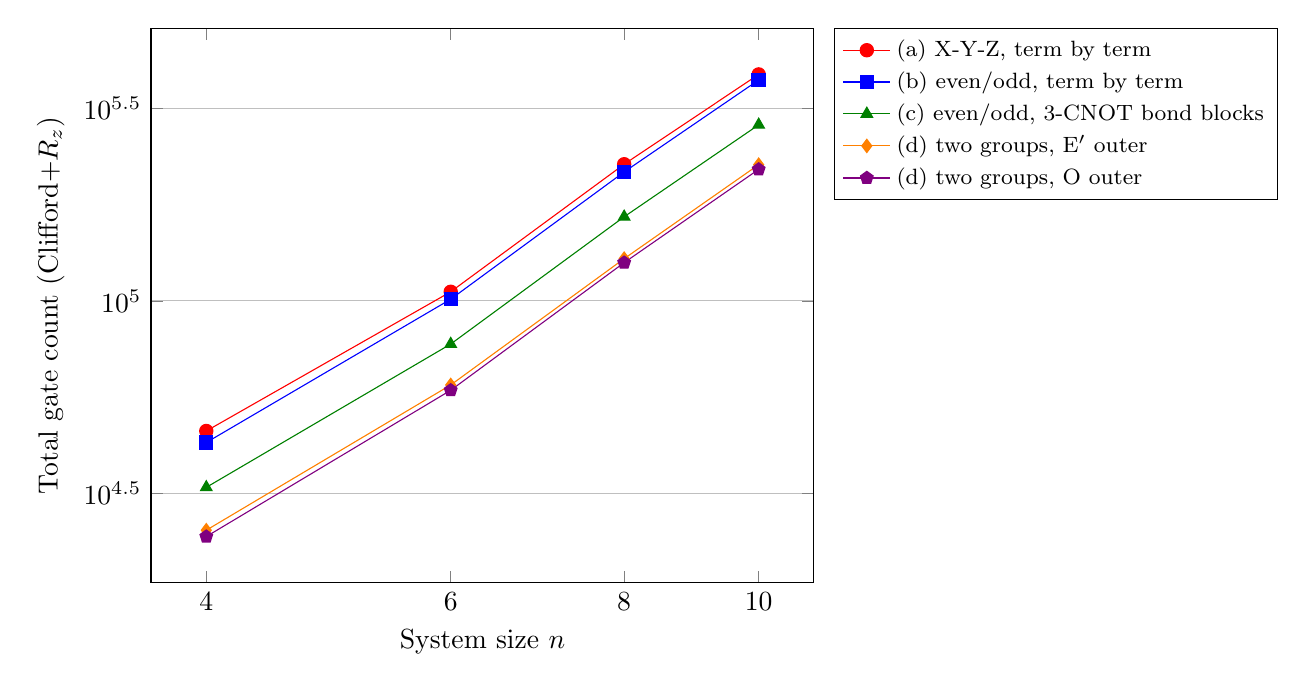
\begin{tikzpicture}
  \begin{loglogaxis}[
    width=10cm,
    xlabel={System size $n$},
    ylabel={Total gate count (Clifford+$R_z$)},
    xtick={4,6,8,10},
    xticklabels={4,6,8,10},
    ymajorgrids=true,
    legend pos=outer north east,
    legend cell align=left,
    legend style={font=\footnotesize},
  ]
    \addplot[red, mark=*, mark size=2.4pt, mark options={solid, fill=red}] coordinates {
      (4,45900)
      (6,105570)
      (8,226440)
      (10,387600)
    };
    \addlegendentry{(a) X-Y-Z, term by term}
    \addplot[blue, mark=square*, mark size=2.4pt, mark options={solid, fill=blue}] coordinates {
      (4,42840)
      (6,100980)
      (8,216240)
      (10,374850)
    };
    \addlegendentry{(b) even/odd, term by term}
    \addplot[green!50!black, mark=triangle*, mark size=2.4pt, mark options={solid, fill=green!50!black}] coordinates {
      (4,32760)
      (6,77220)
      (8,165360)
      (10,286650)
    };
    \addlegendentry{(c) even/odd, 3-CNOT bond blocks}
    \addplot[orange, mark=diamond*, mark size=2.4pt, mark options={solid, fill=orange}] coordinates {
      (4,25350)
      (6,60450)
      (8,128700)
      (10,225875)
    };
    \addlegendentry{(d) two groups, E$'$ outer}
    \addplot[violet, mark=pentagon*, mark size=2.4pt, mark options={solid, fill=violet}] coordinates {
      (4,24400)
      (6,58560)
      (8,125660)
      (10,219600)
    };
    \addlegendentry{(d) two groups, O outer}
  \end{loglogaxis}
\end{tikzpicture}
